\documentclass[
11pt,%
tightenlines,%
twoside,%
onecolumn,%
nofloats,%
nobibnotes,%
nofootinbib,%
superscriptaddress,%
noshowpacs,%
centertags]%
{revtex4}
\usepackage{ljm}
\usepackage{listings}
\usepackage{amsmath}

\lstset{
language=C++,
basewidth=0.5em,
xleftmargin=45pt,
xrightmargin=45pt,
basicstyle=\small\ttfamily,
keywordstyle=\bfseries\underbar,
numbers=left,
numberstyle=\tiny,
stepnumber=1,
numbersep=10pt,
showspaces=false,
showstringspaces=false,
showtabs=false,
frame=trBL,
tabsize=2,
captionpos=t,
breaklines=true,
breakatwhitespace=false,
escapeinside={\%*}{*)}
}

\begin{document}

\titlerunning{Scaling of supercomputer calculations}
\authorrunning{Shabanov et al.}

\title{Scaling supercomputer computations on unstructured surface computational meshes}

\author{\firstname{B.~M.}~\surname{Shabanov}}
\email[E-mail: ]{shabanov@jscc.com}
\affiliation{Joint Supercomputer Center of the Russian Academy of Sciences -- branch of Scientific Research Institute of System Analysis of the Russian Academy of Sciences, Leninsky prospect 32a, Moscow, 119334, Russia}

\author{\firstname{A.~A.}~\surname{Rybakov}}
\email[E-mail: ]{rybakov.aax@gmail.com}
\affiliation{Joint Supercomputer Center of the Russian Academy of Sciences -- branch of Scientific Research Institute of System Analysis of the Russian Academy of Sciences, Leninsky prospect 32a, Moscow, 119334, Russia}

\author{\firstname{S.~S.}~\surname{Shumilin}}
\email[E-mail: ]{noisd@yandex.ru}
\affiliation{Joint Supercomputer Center of the Russian Academy of Sciences -- branch of Scientific Research Institute of System Analysis of the Russian Academy of Sciences, Leninsky prospect 32a, Moscow, 119334, Russia}

\author{\firstname{M.~Yu.}~\surname{Vorobyov}}
\email[E-mail: ]{nordmike@jscc.com}
\affiliation{Joint Supercomputer Center of the Russian Academy of Sciences -- branch of Scientific Research Institute of System Analysis of the Russian Academy of Sciences, Leninsky prospect 32a, Moscow, 119334, Russia}

\firstcollaboration{(Submitted by A.~M.~Elizarov)} % Add if you know submitter.
%\lastcollaboration{ }

\received{TODO}

\begin{abstract}
When solving complex problems of numerical modeling, computational meshes, containing hundreds of millions of cells are quite often.
Modern tasks even cross the line of billion cells.
Workstations are unable to cope with such volume of data and computation.
To perform computations of this volume we need to use supercomputer clusters consisting of many computational nodes interconnected by a high-speed communication network.
In this case, it is necessary to perform the decomposition of the computational mesh into separate domains in order to ensure its parallel processing on all nodes of the cluster.
These domains are distributed among the computational nodes of the supercomputer and are processed independently of each other.
To efficiently perform computations and scale them to a large number of computational nodes, it is necessary to develop efficient algorithms for decomposition of computational meshes that generate many domains with imposed requirements.
We consider a hierarchical decomposition algorithm with the choice of the optimal criterion for dividing mesh into domains.
As such a mesh we study an unstructured surface mesh used to calculate the processes of interaction of a volumetric body with the environment.
Using this decomposition algorithm, supercomputer calculations are performed on the computing resources of JSCC RAS in order to measure the practical indicators of scalability of highly loaded applications.
\end{abstract}

\subclass{65Y05,65Y20,49M27} % Enter 2010 Mathematics Subject Classification.

\keywords{supercomputer,  unstructured surface computational mesh, decomposition, domain, high-performance computing, scaling of calculations}

\maketitle

\section{Introduction}

Modern computational applications are extremely demanding on computational resources.
For large tasks it is not possible to execute them on a separate computer (one microprocessor or one server) in reasonable time.
There is a need to use supercomputer clusters for computations, consisting of many computational nodes.
In order to perform a task on a supercomputer, it is necessary to divide its computational domain into separate subdomains and process them in parallel.

To improve the efficiency of supercomputer applications within a computing node, various methods of data preparation and parallelization of execution for systems with shared memory are used.
Low-level optimizations of program code, such as vectorization, which can significantly increase the speed of application execution can also be very efficient.
Of course, at the boundaries of domain contact, it becomes necessary to synchronize computations, which is achieved by data exchange (for example, using MPI).

Thus, the execution of supercomputer calculations consists of two alternating steps: parallel processing of cells of the computational domain and data exchange at the boundaries of contact of domains.
The efficiency of supercomputer applications execution essentially depends on the quality of the computational mesh decomposition and its distribution over different computational nodes.

This article studies the problem of decomposition of surface unstructured computational mesh for distribution between the nodes of homogeneous supercomputer cluster  to increase the efficiency of computational scaling.
By homogeneous we mean a cluster consisting of the same computational nodes.

Take a surface mesh consisting of $ S $ computational cells.
Let the supercomputer consist of $ n $ computational nodes with the same characteristics.
We will also assume that the speed of data exchange between any two computational nodes is the same for all nodes.
Extension of the problem of distributing the computational load to a heterogeneous computational cluster is achieved by entering weights for computational nodes and for data exchange channels, as described in [TODO].

If we represent the processing speed of computational cells on one computational node as $ a^{-1} $, then the execution time of one iteration of computations on one computational node will be equal to $ T_1 = aS $.
Now let the computational domain be divided into $ n $ domains each containing $ S_i $ cells ($ i = 1, n $).
Let us denote by $ L_{ij} $ the number of edges that form the border between the domains $ S_i $ and $ S_j $.
We will assume that each domain is processed on its own computational node.
Thus, all domains are processed in parallel, and the processing time for all cells is determined by the processing time for the largest domain.
In addition to processing all computational cells, after a calculation iteration, it is necessary to exchange data between all pairs of domains along their boundaries.
Let the speed of data transfer between nodes be determined as $ b^{-1} $, and all exchanges are performed in parallel.
Then the execution time of all exchanges is determined by the time of data exchange across the longest boundary.
Based on this, it is possible to determine the total execution time of one iteration of calculation when executing on $ n $ computational nodes:

\begin{equation}
T_n = a \max_{i = 1,n}{S_i} + b \max_{i,j=1,n}{L_{ij}}.
\end{equation}

The criterion for optimization of computational mesh's decomposition is the reduction of time for performing calculations, that is, the value of $ T_n $.
The calculation execution time directly depends on the size of the largest domain, however, we will consider not the absolute size of the domain, but its deviation from the theoretical optimal value.
Obviously, in the ideal case, during decomposition, all domains should have the size $ \frac{S}{n} $, and the relative deviation from the ideal size in percentage can be calculated by the formula:

\begin{equation}
D = 100 \% \left( \frac{n}{S} \max_{i=1,n}{S_i} - 1 \right).
\end{equation}

The second important criterion for the quality of the performed decomposition is the longest length of the boundary between pairs of domains.
In this case, the absolute characteristic can be used, since the length of the boundary is rather difficult to predict, and generally speaking, it has no theoretical minimum.
Depending on the geometry of the mesh under consideration, the length of the boundary between domains can theoretically be zero.
We will use the following value as metric for comparing various mesh decomposition methods:

\begin{equation}
L = \max_{i,j=1,n}{L_{ij}}.
\end{equation}

Despite the fact that, in our assumptions, all data exchanges between domains are executed simultaneously, the total volume of all exchanges significantly affects the data exchange rate, so this parameter must also be taken into account.
Let us introduce it in the following form.
The total number of edges in the computational mesh remains unchanged regardless of the decomposition algorithm and number of domains.
We denote the total number of edges in the mesh by $ E $.
Among these edges there are border edges that have only one incident cell, their number is also constant and equal to $ E_B $ (from the word "border").
The rest of the edges have two incident cells.
If both cells incident to a certain edge belong to the same domain, then we call such an edge an inner edge of this domain.
We denote their number by $ E_{INN} $ from the word "inner".
Otherwise the edge enters the boundary between two domains and we call it an interdomain edge.
$ E_{INT} $ is their number.
There can be no other types of edges.
Thus, the relation $ E = E_B + E_{INN} + E_{INT} $ is fulfilled.
As a parameter for evaluating the quality of decomposition, we will consider the fraction of interdomain edges in the total number of mesh edges, that is, the value:

\begin{equation}
I = 100 \% \left( \frac{E_{INT}}{E} \right).
\end{equation}

To assess the quality of the computational mesh decomposition, all three described parameters should be taken into account: $ D $ is the deviation of the biggest domain size from the ideal value, $ I $ is the fraction of interdomain edges in the total number of edges of the computational mesh, and $ L $ is the length of the longest boundary between pairs of domains.
The lower the values of these criteria, the better the decomposition is and the more efficient calculations can be expected when running on a real machine.

\section{Parallelization of computations on an unstructured computational mesh}

\begin{figure}[h]
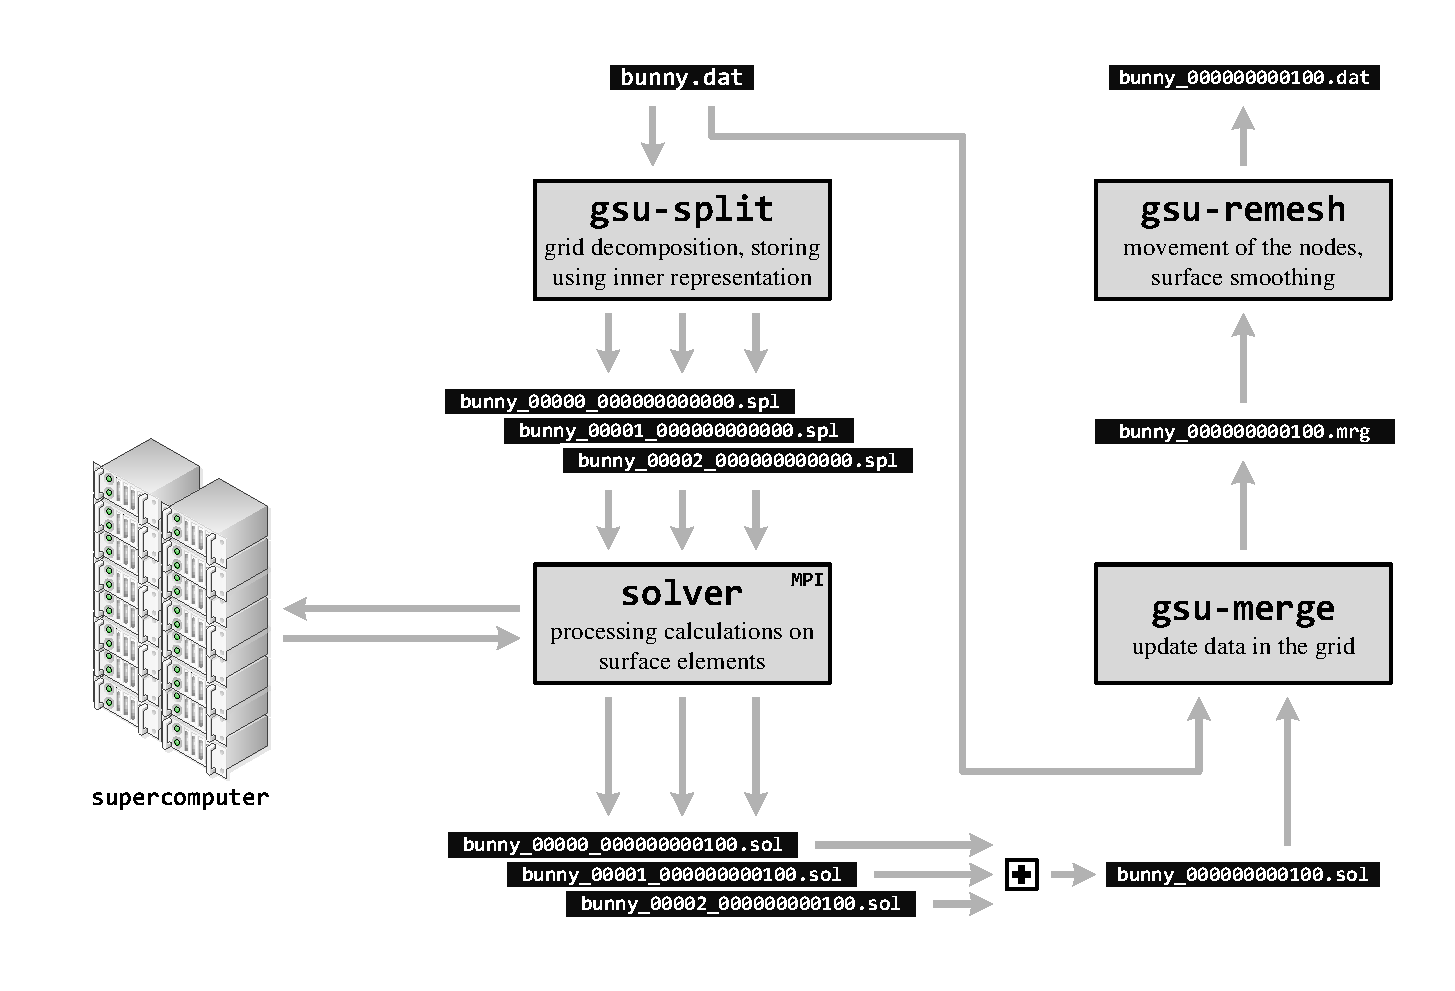
\includegraphics[width=1.0\textwidth]{pics/02-scheme.pdf}
\captionstyle{center}\caption{Parallelization scheme for computations on a supercomputer.}\label{fig:02-scheme}
\end{figure}

Consider a parallelization scheme for computations associated with modeling the interaction of a volumetric body with the environment.
In this case, calculations are carried out on the surface of an interacting body described by an unstructured surface computational mesh (MSU - Mesh Surface Unstructured) with triangular cells.
In the considered calculation scheme on the body surface, various physical processes are considered, including surface deformation, the flow of a liquid film, and ice accretion, which ultimately should lead to remeshing of the calculated surface.
The calculation scheme is thus divided into several independent functional modules (the scheme of interaction of the modules is shown in Fig~\ref{fig:02-scheme}).

The first module -- \texttt{msu-split} -- is designed to load the computational mesh, decompose it into several domains and prepare it for solver.
The physical solver \texttt{solver} is intended only for high-load computations, it interacts with a supercomputer cluster and operates on an arbitrary number of computational nodes.
This is the most resource-demanding part of the application, which takes more than 90 \% of the estimated time, so it is implemented using MPI, OpenMP and vectorization of the program code.
After carrying out the necessary calculations, the \texttt{solver} module returns the accumulated data from different time points, which are fed into the \texttt{msu-merge} data fusion module.
The last link in the chain of calculations is the \texttt{msu-remesh} module, which receives a computational mesh as input (in general case, a set of computational meshes from different points in time) and remeshes it.

\section{Decomposition of an unstructured computational mesh}

[TODO] describes a parallel algorithm for geometric decomposition of mesh data.
During the operation of this algorithm, the current domain is sequentially halved using a plane section.
According to the logic of this algorithm, the initial head domain (\texttt{h} -- head) is halved into a pair of domains \texttt{hl} (left), \texttt{hr} (right), each of which is further halved, and so on up to any number of domains equal to a power of two.

We propose to extend this algorithm by introducing arbitrary criteria for dividing the current domain into a pair of smaller domains.
First, consider the scheme of simple bisection of a domain using an arbitrary criterion by which the division is performed (Fig.~\ref{fig:03-split}).

\begin{figure}[h]
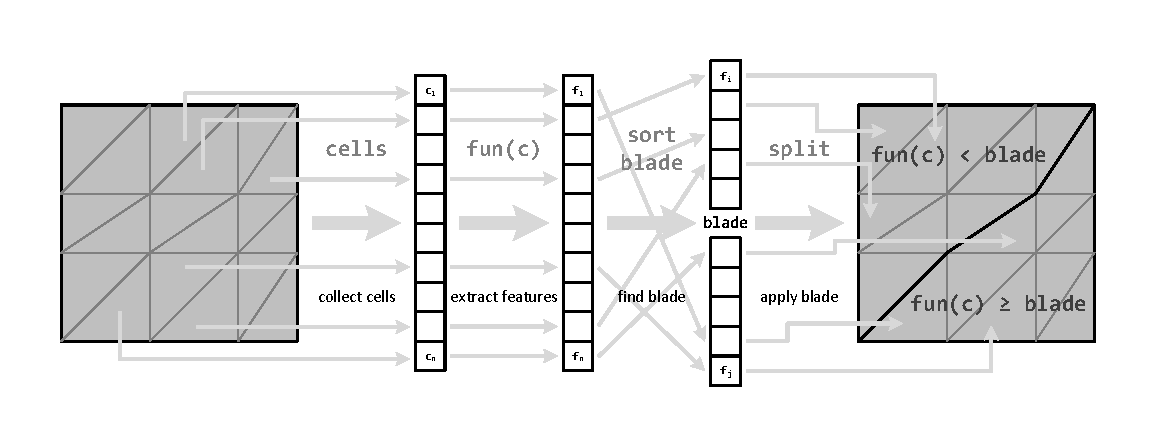
\includegraphics[width=1.0\textwidth]{pics/03-split.pdf}
\captionstyle{center}\caption{A scheme of halving the domain according to the selected attribute fun.}\label{fig:03-split}
\end{figure}

Assume a set of cells of domain \texttt{h} and some function \texttt{fun} for extracting a feature from a cell.
The first step is to calculate a set of features for all cells (\texttt{s} -- signs):
\begin{equation*}
	s = \{fun(h_i)~|~h_i \in h\}.
\end{equation*}

Then sort \texttt{s}.

In the sorted set of features, the median value should be chosen (\texttt{b} -- blade):
\begin{equation*}
	b = median(s).
\end{equation*}

This value will be used to split the domain into two smaller domains (\texttt{hl} -- head left, \texttt{hr} -- head right) using two simple filters:
\begin{equation*}
	hl = \{h_i~:~fun(h_i) < b,~h_i \in h\},
\end{equation*}
\begin{equation*}
	hr = \{h_i~:~fun(h_i) \geq b,~h_i \in h\}.
\end{equation*}

After splitting a domain into two smaller domains, you can calculate a parameter that reflects the efficiency of splitting.
We propose to use the length of the boundary between the two newly formed domains as such a parameter.
Thus, the splitting criterion depends on the function of calculating the attribute \texttt{fun}.
In turn, this means that when performing a partition, it is not necessary to be limited to one function of calculating a feature.
Instead, you can submit a list of functions, for each function calculate the parameter of quality of the partition and, as a result, stop at the function, which ultimately leads to the most efficient partition.

If we simply use the extraction of the three coordinates of the cells' centers as functions for calculating the feature of a cell, then we will obtain in its pure form an algorithm for the geometric decomposition of the mesh with the choice of longest coordinate for splitting.
The results of applying this algorithm can be seen in Fig.~\ref{fig:03-explode-bunny} and Fig.~\ref{fig:03-hierarch}.

\begin{figure}[h]
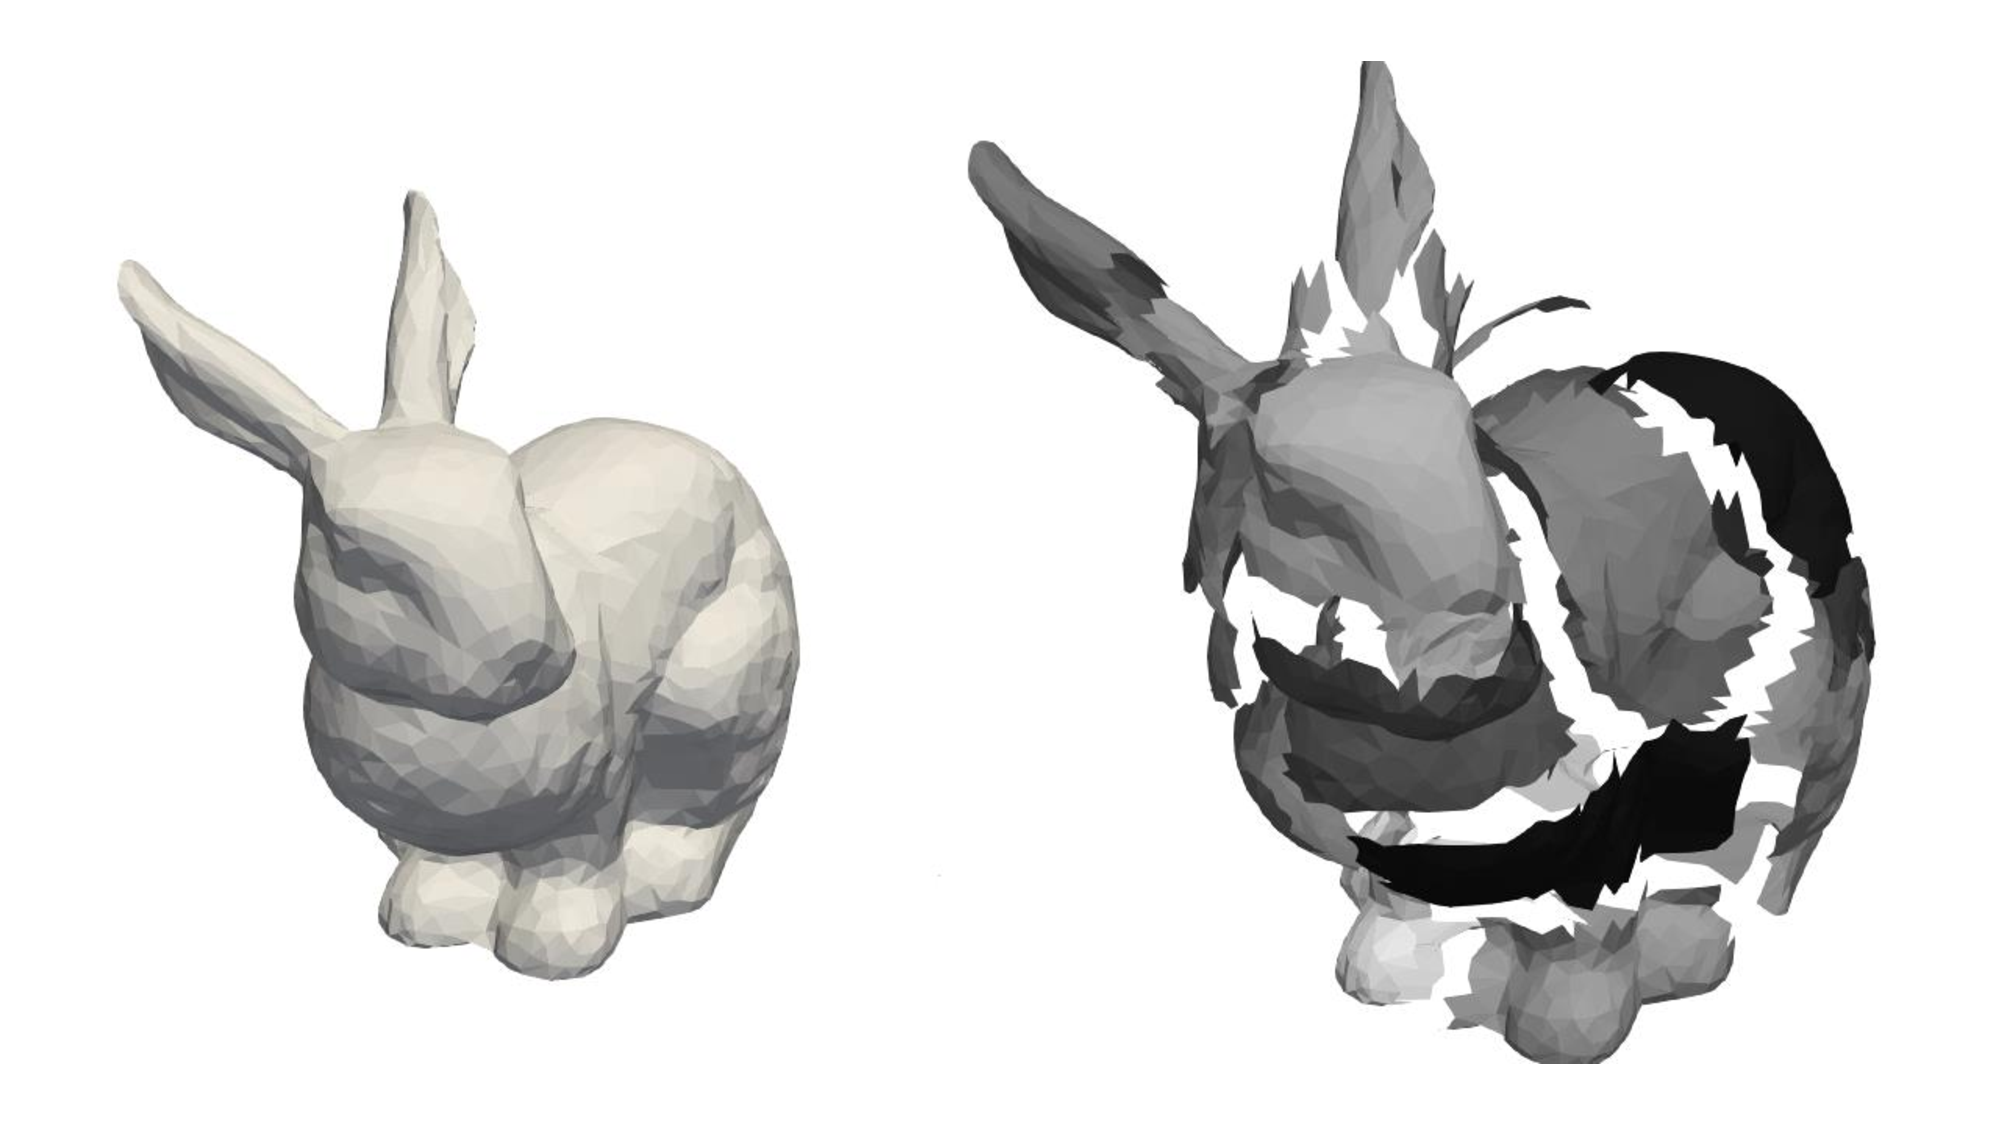
\includegraphics[width=1.0\textwidth]{pics/03-explode-bunny.pdf}
\captionstyle{center}\caption{An example of decomposition of a surface computational mesh using a hierarchical algorithm.}\label{fig:03-explode-bunny}
\end{figure}

\begin{figure}[h]
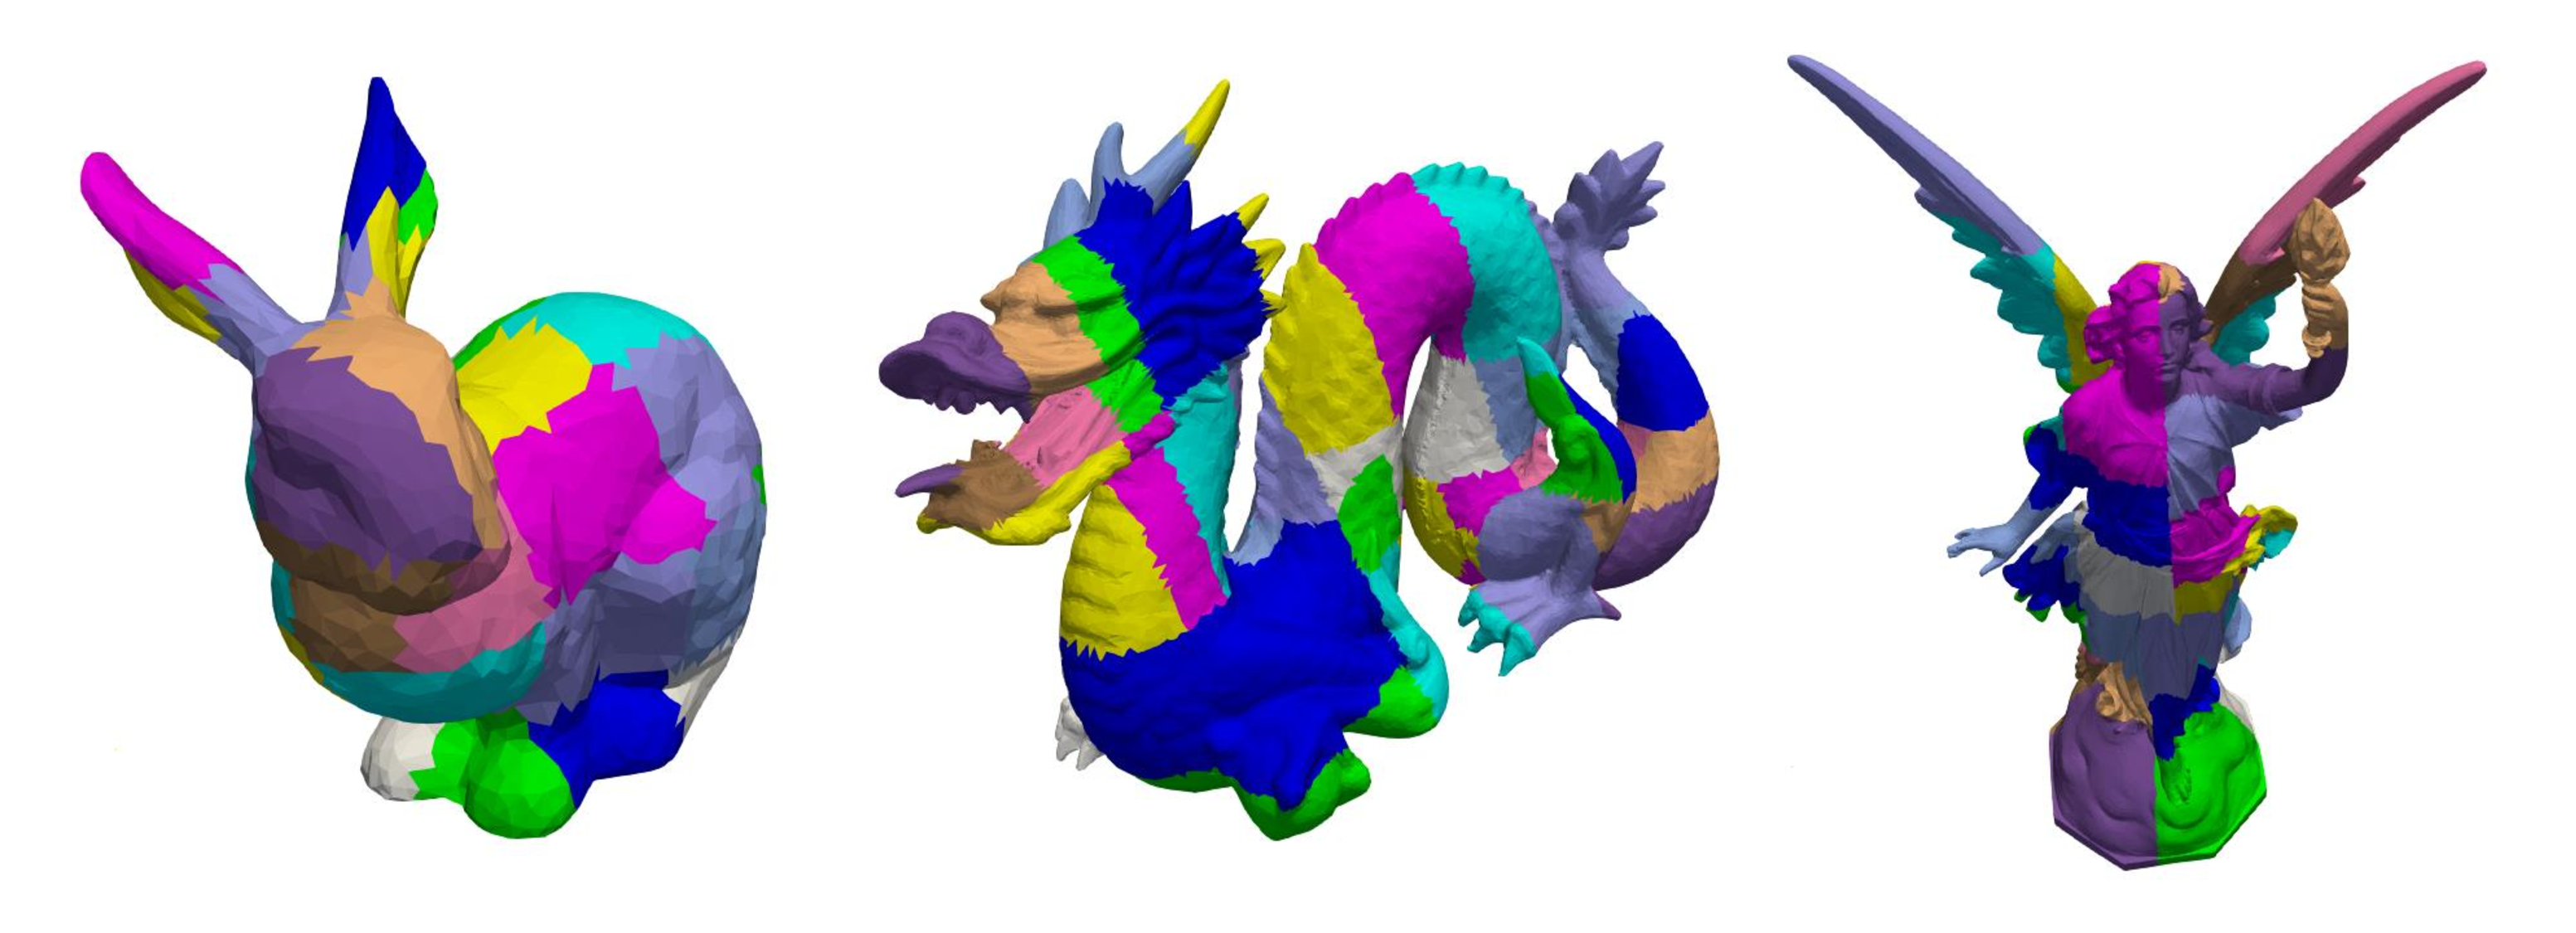
\includegraphics[width=1.0\textwidth]{pics/03-hierarch.pdf}
\captionstyle{center}\caption{Examples of surface computational mesh decomposition using a hierarchical algorithm.}\label{fig:03-hierarch}
\end{figure}

By varying set of features for choosing those by which the domain can be partitioned, it is possible to perform geometric decomposition along the direction of any curve for which the cell projection is calculated.
Decomposition using this method is not limited to geometric features only.
Feature calculating functions can be used to analyze the physical data of cells, for example, to localize and isolate areas with increased pressure into separate domains.

Within the framework of this work, the described algorithm for decomposition of the surface unstructured computational mesh was applied to the surface meshes used to calculate icing of the aircraft surface.
When calculating icing of an aircraft, the bulk of the computations relates to the processing of surface cells.
Shared data between adjacent domains is collected on interdomain edges.
The typical size of such meshes was about $ 10^5 $ cells. We considered both simply connected and not simply connected surfaces, as well as surfaces consisting of several zones isolated from each other.

It should be noted that the theoretical quality parameters $ D $, $ L $, $ I $ are quite low.
The $ D $ parameter is practically zero, since at each step the domain is divided strictly in half.
The deviations in the lengths of the boundaries between domains and the total length of the boundaries are also acceptable, despite the fact that the algorithm does not guarantee the formation of domains with minimal boundaries or even connected domains
In the worst cases, domains of arbitrary shape and consisting of an arbitrary number of isolated parts of the surface may arise.
Of course, a significant limitation of the algorithm is that it can be used to partition the surface only into the number of parts, which is a power of two, but the close-to-zero value of the computational load balancing quality index $ D $ allows in this case to neglect this drawback.

\section{Organization of interprocess exchanges}

\begin{figure}[h]
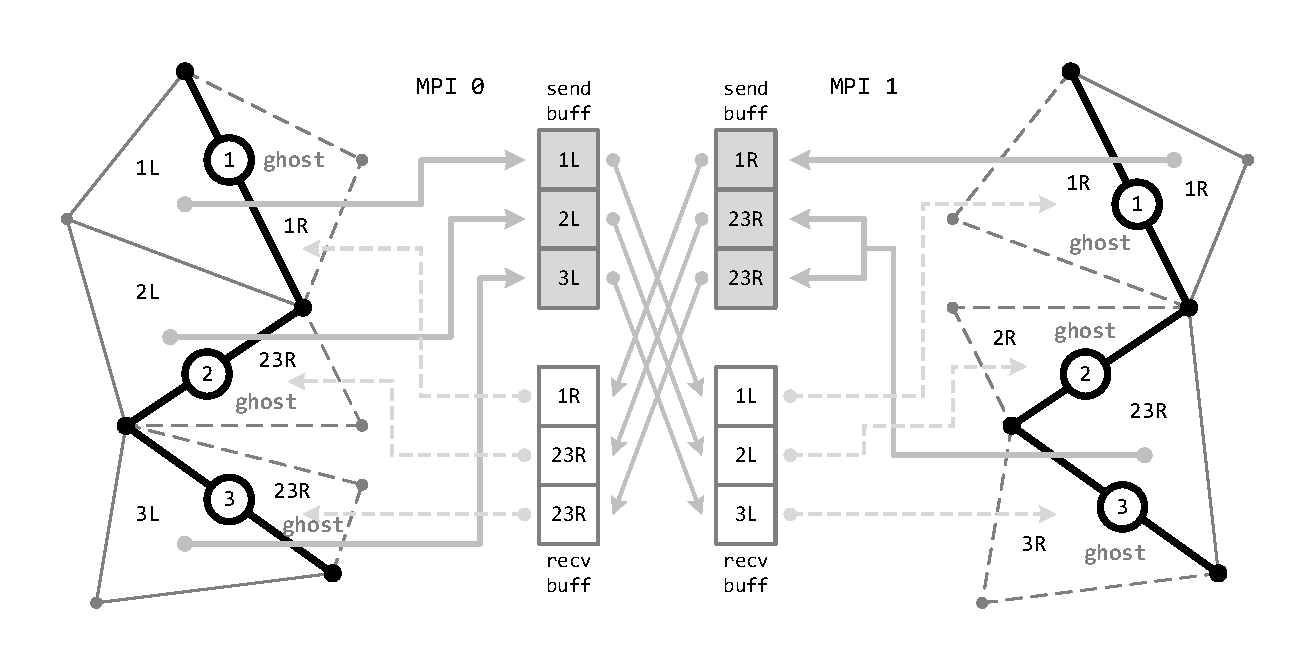
\includegraphics[width=1.0\textwidth]{pics/04-MPI.pdf}
\captionstyle{center}\caption{Scheme of execution of MPI-exchanges across the border of two zones.}\label{fig:04-MPI}
\end{figure}

When performing calculations on a decomposed mesh, at each iteration of the computation, it is necessary to exchange data at each boundary between domains.
In our case, when performing the decomposition of the computational mesh, the boundary between two domains is represented by an arbitrary set of interdomain edges.
In this case, the boundary may be discontinuous, it may even consist of separate edges, therefore the sequence of interdomain edges is not important when describing the boundary.

Fig.~\ref{fig:04-MPI} shows a scheme of organization of interprocess exchanges.
Two domains (we will conventionally call them left and right), processed in MPI processes numbered 0 and 1, are separated by a boundary consisting of three edges.
In this case, there are three cells in the left domain that are adjacent to the considered boundary, in the right domain there are only two such cells (since cell 23R is adjacent to two edges of the boundary at once).
To organize interprocess communications in each domain, ghost cells are created for each edge of the considered boundary, which are involved in calculating flows through the edges.
At the same time, there is no need to recalculate physical values in ghost cells
All data for ghost cells is obtained using MPI exchanges from real cells of a neighboring domain.

To transfer data from the real border cells of the domain to the ghost cells of the neighboring domain, buffers for sending and receiving data are organized in each of the two neighboring domains.
The data exchange sequence is as follows (the diagram is shown in Fig.~\ref{fig:04-MPI}).
First, data from real boundary cells is written to the corresponding send buffers (send buff), then asynchronous commands \texttt{MPI\_Irecv} for receiving messages in the data receiving buffers (recv buff) are executed for all boundaries of the computational mesh.
After that, commands for asynchronous sending of data \texttt{MPI\_Isend} from the send buffers are also executed simultaneously for all boundaries of the computational mesh.
Next, it waits for the completion of all asynchronous data exchanges using the \texttt{MPI\_Waitall} function.
The last step, completing the exchange of data between neighboring domains, is the transfer of the received physical values from the data receiving buffers (recv buff) to the corresponding ghost cells.

Note that some data duplication may occur when using ghost cells.
For example, in the presented diagram, cell 23R from the right domain corresponds at once to two ghost cells in the left domain.
These cells contain the same data.
This duplication of information is acceptable, since the data of the ghost cells is used only for reading to perform the calculation of flows across the domain boundary, therefore, in this case, there is no need to perform any synchronization of the same ghost cells.

\section{Efficiency of scaling supercomputer computations}

To measure the scalability of computations on an unstructured surface computational mesh, a test surface of a streamlined three-dimensional body was used, containing about $ 2 \cdot 10^5 $ nodes and $ 4 \cdot 10^5 $ cells.
In the cells, calculations were performed related to modeling the flow of a liquid film, solving the heat balance equations on the surface, as well as remeshing and smoothing the surface.
To decompose the surface mesh, we used a simple hierarchical algorithm for halving domains, in which three coordinates of the center were taken as the features of the cells.
At the same time, as a result, the criterion for choosing a specific coordinate for dividing a domain was to minimize the length of the boundary between two domains (this approach allows dividing a domain along the longest direction).

\begin{table}[!h]
\label{tbl:supercomputers}
\setcaptionmargin{0mm}
\onelinecaptionsfalse
\captionstyle{flushleft}
\caption{The configurations of the segments of the MVS-10P OP supercomputer, on which the computation scaling measurements were taken.}
\bigskip
\begin{tabular}{|c|c|c|c|c|}
\hline
\parbox{3.5cm}{\textit{Family of\\Intel microprocessors}} & \parbox{4.0cm}{\textit{Number of\\processors/ cores /\\threads per node}} & \parbox{3.0cm}{\textit{Frequency of\\microprocessor}} & \parbox{3.0cm}{\textit{RAM\\per node}} & \parbox{2.0cm}{\textit{Supports\\AVX-512}} \\
\hline
Xeon Broadwell & 2 / 32 / 64 & 2.6 GHz & 128 GB & no \\
\hline
Xeon Phi KNL & 1 / 72 / 288 & 1.5 GHz & 96 GB & yes \\
\hline
Xeon Skylake & 2 / 36 / 72 & 3.0 GHz & 192 GB & yes \\
\hline
Xeon Cascade Lake & 2 / 48 / 96 & 3.0 GHz & 192 GB & yes \\
\hline
\end{tabular}
\label{tab:supercomputers}
\end{table}   

Homogeneous segments of the computing system of Joint Supercomputer Center of the Russian Academy of Sciences were used to measure the computational scalability.
In total, the calculations were carried out on four computational segments, the characteristics of the nodes of which are given in the table \ref{tab:supercomputers}.
In this table, it can be noted that all microprocessors except Xeon Broadwell support the AVX-512 instruction set, which allows the use of special 512-bit vector registers for efficient code vectorization.
We should also highlight the computing nodes based on the Xeon Phi KNL microprocessor.
These microprocessors are distinguished by a huge number of computing cores, each of which is capable of executing up to 4 threads, which allows efficient parallelization of computational applications up to 288 threads on a single microprocessor.

\begin{figure}[h]
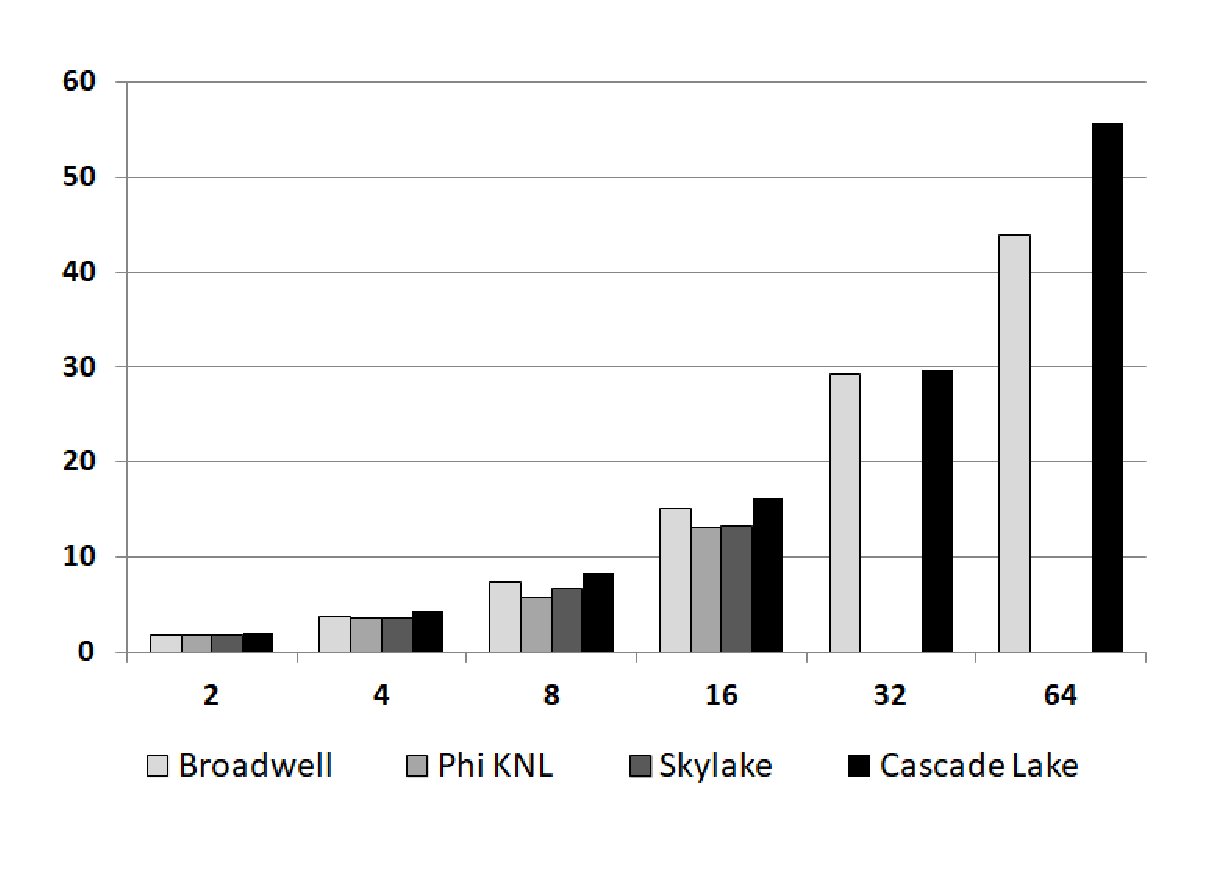
\includegraphics[width=0.8\textwidth]{pics/speedup.pdf}
\captionstyle{center}\caption{Acceleration of computations on supercomputers at JSCC RAS when increasing the number of nodes.}\label{fig:speedup}
\end{figure}

The main goal of the launches was to measure the strong scalability of computations with full parallelization within computational nodes using OpenMP.
That is, for all launches, the same surface was used (which was split over the required number of computational nodes), and all the threads available inside the computational nodes were also involved in the calculations.

When carrying out the calculations, the measurements were carried out independently for each computer system separately.
Let us give a description of the quantities measured in the calculation process for one specific computing system.
The time of the task execution on one computational node was used as the reference time: $ t(1) $.
We also measured the execution time of tasks for the number of computational nodes equal to a power of two (2, 4, 8, 16, 32, 64).
In this case, the acceleration on the number of nodes equal to $ i $ was considered the value of the value $ s(i) = \frac{t(1)}{t(i)} $.
Fig.~\ref{fig:speedup} shows diagrams of computation acceleration with an increase in the number of computational nodes for different computational systems.

In addition to calculating the direct speedup of code execution, calculations of the scaling efficiency were performed.
In this case, the computational scaling efficiency is understood as the value $ e(i) = \frac{s(i)}{i} $.
The physical meaning of it is as follows.
We can assume that in the case of ideal parallelization of computations increasing the number of nodes by $ n $ times, the execution time decreases exactly by $ n $ times.
Thus, in the case of ideal parallelization, $ s (i) = i $, and $ e(i) = 1 $.
The efficiency of scaling computations is a convenient indicator of the quality of creating executable parallel code and comparing different computing systems with each other.
Note that super-linear scalability is quite possible (when the value of $ e(i) $ rises above one), but this is more an exception than an expected effect.

\begin{figure}[h]
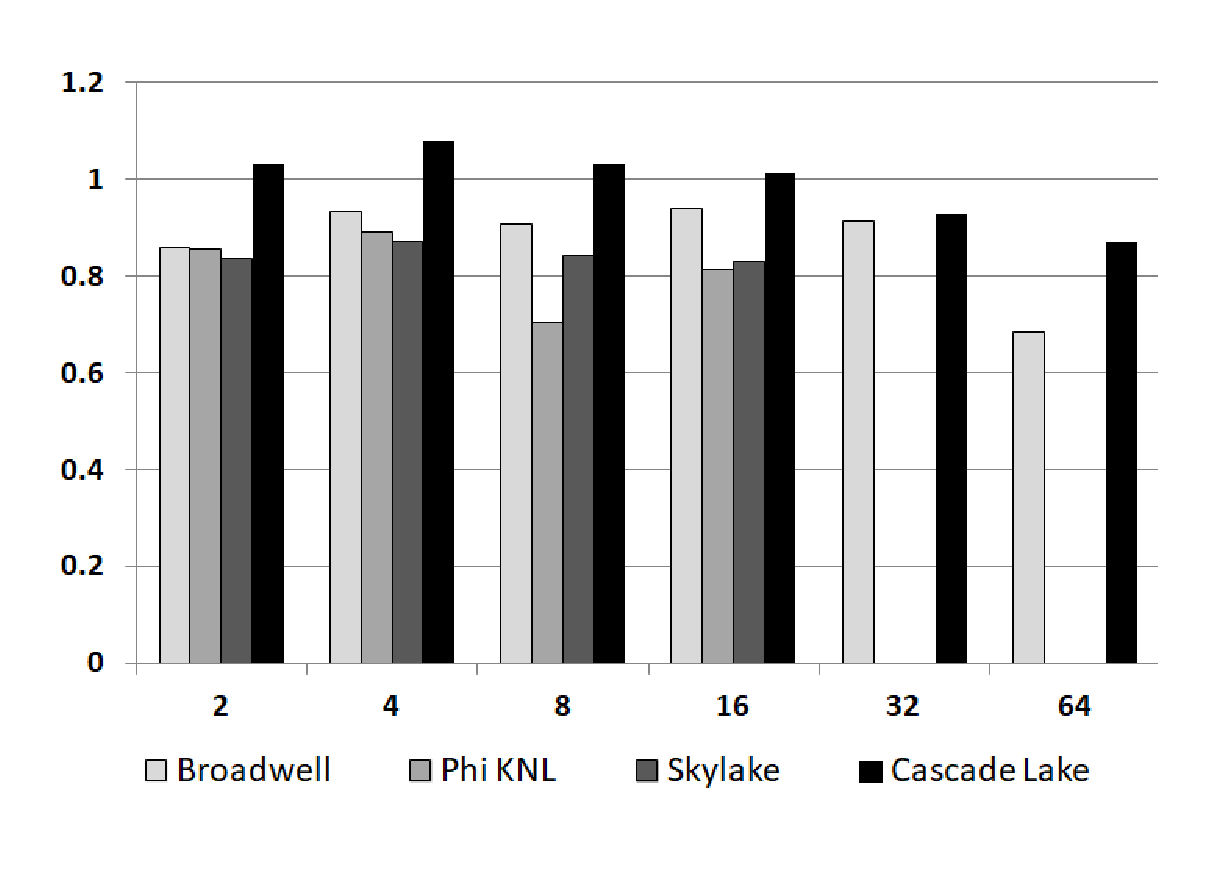
\includegraphics[width=0.8\textwidth]{pics/scaling.pdf}
\captionstyle{center}\caption{Efficiency of scaling computations on supercomputers of JSCC RAS when increasing the number of nodes.}\label{fig:speedup}
\end{figure}

Fig.~\ref{fig:speedup} shows a diagram of the scaling efficiency of computations for various computational segments, depending on the number of computational nodes used.
It can be seen that for all computing systems, the scaling efficiency varies in the region of 0.8-0.9, although on some launch configurations there are dips even in the region of 0.7.
Launches with a low parallelization efficiency are usually associated with a spread in the processing time of MPI processes in their domains.
Despite the fact that the algorithm for decomposition of the computational mesh used in this article provided a uniform distribution of cells across domains, the processing time of a cell itself strongly depends on its physical properties and can differ significantly.
For this reason, balancing the computational load on different computational nodes is possible only in a dynamic mode, which was not done within the framework of this study.
We also note the high efficiency of scaling computations for compute nodes based on Xeon Cascade Lake microprocessors.
These processors are the most modern of all the equipment used in the described experiment.

\section{Conclusion}

The efficiency of scaling high-load computing is an important aspect when developing parallel applications and performing calculations.
Today, given the complexity of scientific and engineering problems and the amount of data being processed, it is difficult to rely on the efficiency of local station or server.
To conduct qualitative research using modern mathematical models, the use of supercomputers is required.
To use them effectively, you need to be able to create applications that can run in parallel on many computing nodes.
To assess the efficiency of running parallel applications, it is convenient to use an indicator called the efficiency of computing scaling, the proximity of which to 1 indicates that the approaches and methods used for organizing high-performance computing reasonably reflect the needs of the problem and hardware.
This article describes various aspects that are critical to achieving high compute scaling efficiency.
Among them are the decomposition of the computational mesh, the mechanism for organizing interprocess exchanges during the counting process, and building the entire chain of calculations into a single sequence of actions.
To obtain practical results in the course of the study, the problem of calculating physical processes on the surface of a streamlined body was used.
All the work was performed on an unstructured surface computational mesh.
To carry out the launches, several segments of the computing system of JSCC RAS were used.
The highest computation scaling efficiency among which was achieved on the segment based on Xeon Cascade Lake microprocessors.

\begin{acknowledgments}
The work has been done at the JSCC RAS as part of the state assignment for the topic 0580-2021-0016.
The supercomputer MVS-10P OP (Broadwell, KNL and Cascade Lake segments), located at the JSCC RAS, was used during the research.
\end{acknowledgments}

\begin{thebibliography}{99}

\bibitem{Rettinger}
\refitem{article}
C. Rettinger, C. Godenschwager, S. Eibl, et al., {\it ``Fully Resolved Simulations of Dune Formation in Riverbeds"}, ISC High Performance , LNCS~{\bf 10266}, 3--21 (2017).

\bibitem{Krappel}
\refitem{article}
T. Krappel, S. Riedelbauch, {\it ``Scale Resolving Flow Simulations of a Francis Turbine Using Highly Parallel CFD Simulations"}, High Performance Computing in Science and Engineering'16, 499--510 (2016).

\bibitem{Markidis}
\refitem{article}
S. Markidis, I. B. Peng, J. L. Tr\"aff, et al.,{\it ``The EPiGRAM Project: Preparing Parallel Programming Models for Exascale"}, ISC High Performance Workshops, LNCS~{\bf 9945}, 56--68  (2016).

\bibitem{Klenk}
\refitem{article}
B.~Klenk, H.~Fr\"oning, {\it ``An Overview of MPI Characteristics of Exascale Proxy Applications"}, ISC High Performance, LNCS~{\bf 10266}, 217--236  (2016).

\bibitem{Abduljabbar}
\refitem{article}
M.~Abduljabbar, G.~S.~Markomanolis, H.~Ibeid, et al., {\it ``An Overview of MPI Characteristics of Exascale Proxy Applications"}, ISC High Performance, LNCS~{\bf 10266}, 79--96 (2017).

\bibitem{Rybakov}
\refitem{article}
A.~A.~Rybakov, {\it ``Inner respresentation and crossprocess exchange mechanism for block-structured grid for supercomputer calculations"}, Program systems: Theory and Application~{\bf 32}(8:1), 121--134 (2017).

\bibitem{Van}
\refitem{article}
R.~F.~Van der Wijngaart, E.~Georganas,~T.~G.~Mattson, et al., {\it ``A New Parallel Research Kernel to Expand Research on Dynamic Load-Balancing Capabilities"}, ISC High Performance, LNCS~{\bf 10266}, 256--274 (2017).

\bibitem{Benderskiy}
\refitem{article}
L.~A.~Benderskiy, D.~A.~Lyubimov, A.~A.~Rybakov, {\it ``Analysis of scaling efficiency in high-speed turbulent flow calculations on a RANS / ILES supercomputer using the high resolution method"}, Trudy SRISA RAS~{\bf 7}(4), 32--40 (2017).

\bibitem{Heller}
\refitem{article}
T.~Heller, H.~Kaiser, P.~Diehl et al., {\it ``Closing the Performance Gap with Modern C++"}, ISC High Performance, LNCS~{\bf 9945}, 18--31 (2016).

\bibitem{Roganov}
\refitem{article}
Roganov V., Osipov V., Matveev G., {\it ``Solving the 2D Poisson PDE by Gauss-Seidel method with parallel programming system"}, Program systems: theory and applications~{\bf 30}(7:3), 99--107 (2016).

% References for REVIEW OF RESEARCH PAPERS section.

\bibitem{Jeffers_KNL}
\refitem{book}
J.~Jeffers, J.~Reinders, A.~Sodani, \emph{Intel Xeon Phi Processor High Performance Programming, Knights Landing Edition} (Morgan Kaufmann, 2016).

\bibitem{Jeffers_KNC}
\refitem{book}
J.~Jeffers, J.~Reinders, \emph{Intel Xeon Phi Coprocessor Processor High Performance Programming} (Morgan Kaufmann, 2013).

\bibitem{Dorris}
\refitem{article}
J.~Dorris, J.~Kurzak , P.~Luszczek, {\it ``Task-Based Cholesky Decomposition on Knights Corner Using OpenMP"}, ISC High Performance, LNCS~{\bf 9945}, 544--562 (2016).

\bibitem{Tobin}
\refitem{article}
J.~Tobin, A.~Breuer, A.~Heinecke et al., {\it ``Accelerating Seismic Simulations Using the Intel Xeon Phi Knights Landing Processor"}, ISC High Performance, LNCS~{\bf 10266}, 139--157 (2017).

\bibitem{McDoniel}
\refitem{article}
W.~McDoniel, M.~Hohnerbach, R.~Canales et al., {\it ``LAMMPS' PPPM Long-Range Solver for the Second Generation Xeon Phi"}, ISC High Performance, LNCS~{\bf 10266}, 61--78 (2017).

\bibitem{Malas}
\refitem{article}
T.~Malas, T.~Kurth, J.~Deslippe, {\it ``Optimization of the Sparse Matrix-Vector Products of an IDR Krylov Iterative Solver in EMGeo for the Intel KNL Manycore Processor"}, ISC High Performance, LNCS~{\bf 9945}, 378--389 (2016).

\bibitem{Krzikalla}
\refitem{article}
O.~Krzikalla, F.~Wende, M.~H\"ohnerbach, {\it ``Dynamic SIMD Vector Lane Scheduling"}, ISC High Performance, LNCS~{\bf 9945}, 354--365 (2016).

\bibitem{Cook}
\refitem{article}
B.~Cook, P.~Maris,M.~Shao, {\it ``High Performance Optimizations for Nuclear Physics Code MFDn on KNL"}, ISC High Performance, LNCS~{\bf 9945}, 366--377 (2016).

\bibitem{Rybakov_Optimization}
\refitem{article}
A.~A.~Rybakov,{\it ``Optimization of the problem of conflict detection with dangerous aircraft movement areas to execute on Intel Xeon Phi"}, Programmnye produkty i sistemy [Software \& Systems]~{\bf 30}(3), 524--528 (2017).

\bibitem{Sengupta}
\refitem{article}
D.~Sengupta,~Y.~Wang,~N.~Sundaram et al., {\it ``Performance Incremental SVM Learning on Intel Xeon Phi Processors"}, ISC High Performance, LNCS~{\bf 10266}, 120--138 (2017).

\bibitem{Kronbichler}
\refitem{article}
M.~Kronbichler,~K.~Kormann ,~I.~Pasichnyk, {\it ``Fast Matrix-Free Discontinuous Galerkin Kernels on Modern Computer Architectures"}, ISC High Performance, LNCS~{\bf 10266}, 237--255 (2017).

\bibitem{Doerfler}
\refitem{article}
D.~Doerfler,~J.~Deslippe ,~S.~Williams, {\it `Applying the Roofline Performance Model to the Intel Xeon Phi Knights Landing Processor"}, ISC High Performance, LNCS~{\bf 9945}, 339--353 (2016).

\bibitem{Rosales}
\refitem{article}
C.~Rosales, J.~Cazes, K.~Milfeld, {\it ``Comparative Study of Application Performance and Scalability on the Intel Knights Landing Processor"}, ISC High Performance, LNCS~{\bf 9945}, 307--318 (2016).

% References for FLAT CYCLES section.

\bibitem{Intel_SDM}
\refitem{manual}
Intel 64 and IA-32 Architectures Software Developer's Manual, Combined Volumes: 1, 2A, 2B, 2C, 2D, 3A, 3B, 3C, 3D and 4, Intel Corporation (2017).

\bibitem{Intel_C}
\refitem{manual}
Intel C++ Compiler 16.0 User and Reference Guide, Intel Corporation (2016).

\bibitem{Intel_Intr}
\refitem{misc}
Intel Intrinsics Guide. \url{https://software.intel.com/sites/landingpage/IntrinsicsGuide/}. Accessed 2018.

\bibitem{Scott_Predct}
\refitem{article}
S.~A.~Mahlke, D.~C.~Lin, W.~Y.~Chen, R.~E.~Hank, {\it ``Effective Compiler Support for Predicated Execution Using the Hyperblock"}, Proceedings of the 25th International Symposium on Microarchitecture, ~45--54 (1992).

\bibitem{Hwu_Predct}
\refitem{article}
W.~W.~Hwu, {\it ``The Superblock: an Effective Technique for VLIW and Superscalar Compilation"}, The Journal of Supercomputing~{\bf 7}(1/2), ~229--248 (1993).

\bibitem{Golub}
\refitem{book}
G.~H.~Golub, C.~F.~Van Loan, {\it ``Matrix Computations"}, (The John Hopkins University Press, 1989).

\bibitem{Zhang}
\refitem{article}
H.~Zhang, R.~T.~Mills, K.~Rupp, B.~F.~Smith, {\it ``Vectorized Parallel Sparse Matrix-Vector Multiplication in PETSc Using AVX-512"}, Proceedings of the 47th International Conference on Parallel Processing (ICPP 2018), ACM, Article 55, 10 pages (2018).

\bibitem{Lyub_RANS_ILES}
\refitem{article}
D.~A.~Lyubimov, {\it ``Development and Application of a High-Resolution Technique for Jet Flow Computation Using Large Eddy Simulation"}, High Temperature~{\bf 50}(3),~420--436 (2012).

\bibitem{Ben_Lyub_Chest_RANS_ILES}
\refitem{article}
L.~A.~Benderskii, D.~A.~Lyubimov, A.~O.~Chestnykh, B.~M.~Shabanov and A.~A.~Rybakov, {\it ``The Use of the RANS/ILES Method to Study the Influence of Coflow Wind on the Flow in a Hot, Nonisobaric, Supersonic Airdrome Jet during Its Interaction with the Jet Blast Deflector"}, High Temperature~{\bf 56}(2),~247--254 (2018).

\bibitem{Aleen}
\refitem{article}
F.~Aleen, V.~P.~Zakharin, R.~Krishnaiyer, G.~Gupta, D.~Kreitzer, C.-S.~Lin, {\it ``Automated Compiler Optimization of Multiple Vector Loads/Stores"}, International Journal of Parallel Programming~{\bf 46}(2),~471--503 (2018).

% References for IRREGULAR ITERATIONS LOOPS section.

\bibitem{Fast_Sort}
\refitem{article}
B.~Bramas, {\it ``Fast Sorting Algorithms Using AVX-512 on Intel Knights Landing"}, arXiv: 1704.08579, Accessed 2018.

\bibitem{Quick_Sort}
\refitem{article}
S.~Gueron, V.~Krasnov, {\it ``Fast Quicksort Implementation Using AVX Instructions"}, The Computer Journal,~{\bf 59}(1),~83--90 (2016).

\bibitem{Quick_Sort_2}
\refitem{article}
B.~Bramas, {\it ``A Novel Hybrid Quicksort Algorithm Vectorized Using AVX-512 on Intel Skylake"}, International Journal of Advanced Computer Science and Applications (IJACSA)~{\bf 8}(10), (2017).

\bibitem{Knuth}
\refitem{book}
D.~E.~Knuth, {\it ``The Art of Computer Programming: Volume 3: Sorting and Searching (2nd Edition)"}, (Addison-Wesley Professional, 1998).

% References for PHYSICAL CALCULATIONS section.

\bibitem{Toro}
\refitem{book}
E.~F.~Toro, {\it ``Riemann Solvers and Numerical Methods for Fluid Dynamics:
A Practical Introduction, 2nd Edition"}, (Springer,1999).

\bibitem{Numerica}
\refitem{misc}
NUMERICA, A Library of Sources for Teaching, Research and Applications, by E.~F.~Toro. \url{https://github.com/dasikasunder/NUMERICA}. Accessed 2018.

\end{thebibliography}

\end{document}
